\documentclass{article}\usepackage[]{graphicx}\usepackage[]{color}
%% maxwidth is the original width if it is less than linewidth
%% otherwise use linewidth (to make sure the graphics do not exceed the margin)
\makeatletter
\def\maxwidth{ %
  \ifdim\Gin@nat@width>\linewidth
    \linewidth
  \else
    \Gin@nat@width
  \fi
}
\makeatother

\definecolor{fgcolor}{rgb}{0.345, 0.345, 0.345}
\newcommand{\hlnum}[1]{\textcolor[rgb]{0.686,0.059,0.569}{#1}}%
\newcommand{\hlstr}[1]{\textcolor[rgb]{0.192,0.494,0.8}{#1}}%
\newcommand{\hlcom}[1]{\textcolor[rgb]{0.678,0.584,0.686}{\textit{#1}}}%
\newcommand{\hlopt}[1]{\textcolor[rgb]{0,0,0}{#1}}%
\newcommand{\hlstd}[1]{\textcolor[rgb]{0.345,0.345,0.345}{#1}}%
\newcommand{\hlkwa}[1]{\textcolor[rgb]{0.161,0.373,0.58}{\textbf{#1}}}%
\newcommand{\hlkwb}[1]{\textcolor[rgb]{0.69,0.353,0.396}{#1}}%
\newcommand{\hlkwc}[1]{\textcolor[rgb]{0.333,0.667,0.333}{#1}}%
\newcommand{\hlkwd}[1]{\textcolor[rgb]{0.737,0.353,0.396}{\textbf{#1}}}%
\let\hlipl\hlkwb

\usepackage{framed}
\makeatletter
\newenvironment{kframe}{%
 \def\at@end@of@kframe{}%
 \ifinner\ifhmode%
  \def\at@end@of@kframe{\end{minipage}}%
  \begin{minipage}{\columnwidth}%
 \fi\fi%
 \def\FrameCommand##1{\hskip\@totalleftmargin \hskip-\fboxsep
 \colorbox{shadecolor}{##1}\hskip-\fboxsep
     % There is no \\@totalrightmargin, so:
     \hskip-\linewidth \hskip-\@totalleftmargin \hskip\columnwidth}%
 \MakeFramed {\advance\hsize-\width
   \@totalleftmargin\z@ \linewidth\hsize
   \@setminipage}}%
 {\par\unskip\endMakeFramed%
 \at@end@of@kframe}
\makeatother

\definecolor{shadecolor}{rgb}{.97, .97, .97}
\definecolor{messagecolor}{rgb}{0, 0, 0}
\definecolor{warningcolor}{rgb}{1, 0, 1}
\definecolor{errorcolor}{rgb}{1, 0, 0}
\newenvironment{knitrout}{}{} % an empty environment to be redefined in TeX

\usepackage{alltt}

% \usepackage[utf8]{inputenc}
\usepackage{amsmath}
\usepackage{fancyhdr}
\usepackage{array}
\usepackage{longtable}
\usepackage{graphicx}
\usepackage{color}
\usepackage[letterpaper, margin=1in]{geometry}
\usepackage{lscape}
\newcommand{\blandscape}{\begin{landscape}}
\newcommand{\elandscape}{\end{landscape}}
\usepackage{dcolumn}
\usepackage{bbm}
\usepackage{threeparttable}
\usepackage{booktabs}
\usepackage{expex}
\usepackage{pdflscape}
\usepackage{rotating, graphicx}
\usepackage{tabulary}
\usepackage{lscape}
\usepackage{makecell}
\usepackage{algorithm}
\usepackage{multirow}
\usepackage{colortbl}
\usepackage{longtable}
\usepackage{array}
\usepackage{multirow}
\usepackage{wrapfig}
\usepackage{float}
\usepackage{pdflscape}
\usepackage{tabu}
\usepackage{threeparttable}

\title{%
Homework 11\\
\large Applied Mutlivariate Analysis}
\date{November 19, 2018}
\author{Emorie Beck}
\IfFileExists{upquote.sty}{\usepackage{upquote}}{}
\begin{document}
\maketitle
% \SweaveOpts{concordance=TRUE}

\section{Workspace}
\subsection{Packages}



\begin{knitrout}
\definecolor{shadecolor}{rgb}{0.969, 0.969, 0.969}\color{fgcolor}\begin{kframe}
\begin{alltt}
\hlkwd{library}\hlstd{(car)}
\hlkwd{library}\hlstd{(knitr)}
\hlkwd{library}\hlstd{(kableExtra)}
\hlkwd{library}\hlstd{(psych)}
\hlkwd{library}\hlstd{(MASS)}
\hlkwd{library}\hlstd{(Rmisc)}
\hlkwd{library}\hlstd{(broom)}
\hlkwd{library}\hlstd{(plyr)}
\hlkwd{library}\hlstd{(tidyverse)}
\end{alltt}
\end{kframe}
\end{knitrout}



\subsection{data}
The file, Set\_9.csv, contains data from a hypothetical sample of Ph.D. job seekers. For each individual in the sample, the file contains a GRE (V+Q) score, the number of publications while in graduate school, the years needed to complete the Ph.D., and the applicant’s sex (0=women, 1=men). The outcome variable is whether or not the applicant was invited for at least one interview (0=no, 1=yes). Use binary logistic regression to answer the following questions.

\begin{knitrout}
\definecolor{shadecolor}{rgb}{0.969, 0.969, 0.969}\color{fgcolor}\begin{kframe}
\begin{alltt}
\hlstd{wd} \hlkwb{<-} \hlstr{"https://github.com/emoriebeck/homeworks/raw/master/multivariate/homeworks/homework11"}

\hlstd{dat} \hlkwb{<-} \hlkwd{sprintf}\hlstd{(}\hlstr{"%s/Set_9(1).csv"}\hlstd{, wd)} \hlopt \hlkwd{read.csv}\hlstd{(.,} \hlkwc{stringsAsFactors} \hlstd{= F)} \hlopt
  \hlkwd{mutate}\hlstd{(}\hlkwc{interview} \hlstd{=} \hlkwd{factor}\hlstd{(interview,} \hlkwc{levels} \hlstd{=} \hlkwd{c}\hlstd{(}\hlnum{0}\hlstd{,}\hlnum{1}\hlstd{),} \hlkwc{labels} \hlstd{=} \hlkwd{c}\hlstd{(}\hlstr{"interview"}\hlstd{,} \hlstr{"no interview"}\hlstd{)))} \hlopt
  \hlkwd{mutate_at}\hlstd{(}\hlkwd{vars}\hlstd{(gre, pubs, years),} \hlkwd{funs}\hlstd{(}\hlkwc{c} \hlstd{=} \hlkwd{as.numeric}\hlstd{(}\hlkwd{scale}\hlstd{(.,} \hlkwc{scale} \hlstd{= F))))}

\hlkwd{head}\hlstd{(dat)}
\end{alltt}
\begin{verbatim}
##    ID sex  gre pubs years    interview    gre_c pubs_c years_c
## 1 122   1 1036    0     5 no interview -260.818 -4.302   -1.09
## 2   1   1 1311    0     6    interview   14.182 -4.302   -0.09
## 3 191   0 1196    0     6    interview -100.818 -4.302   -0.09
## 4 194   0 1154    0     6    interview -142.818 -4.302   -0.09
## 5   4   1 1259    0     7    interview  -37.818 -4.302    0.91
## 6   6   1 1308    0     7    interview   11.182 -4.302    0.91
\end{verbatim}
\end{kframe}
\end{knitrout}

\section{Question 1}
Test a model that includes sex, publications, years to complete degree, and GRE score as predictors. For each significant predictor, construct a graph that shows the relationship between that predictor (over its range) and the probability of getting an interview. When constructing graphs, hold non graphed variables constant at their grand means.

\begin{knitrout}
\definecolor{shadecolor}{rgb}{0.969, 0.969, 0.969}\color{fgcolor}\begin{kframe}
\begin{alltt}
\hlstd{fit1}  \hlkwb{<-} \hlkwd{glm}\hlstd{(interview} \hlopt{~} \hlstd{sex} \hlopt{+} \hlstd{gre} \hlopt{+} \hlstd{pubs} \hlopt{+} \hlstd{years,} \hlkwc{data} \hlstd{= dat,} \hlkwc{family} \hlstd{=} \hlkwd{binomial}\hlstd{(}\hlstr{"logit"}\hlstd{))}
\hlkwd{cbind}\hlstd{(}\hlkwd{data.frame}\hlstd{(}\hlkwc{b} \hlstd{=} \hlkwd{coef}\hlstd{(fit1)),} \hlkwd{confint}\hlstd{(fit1))} \hlopt \hlkwd{data.frame}\hlstd{()} \hlopt
  \hlkwd{mutate}\hlstd{(}\hlkwc{term} \hlstd{=} \hlkwd{rownames}\hlstd{(.))} \hlopt
  \hlstd{tbl_df} \hlopt
  \hlkwd{select}\hlstd{(term,} \hlkwd{everything}\hlstd{())} \hlopt
  \hlkwd{setNames}\hlstd{(}\hlkwd{c}\hlstd{(}\hlstr{"term"}\hlstd{,} \hlstr{"b"}\hlstd{,} \hlstr{"lower"}\hlstd{,} \hlstr{"upper"}\hlstd{))} \hlopt
  \hlkwd{mutate}\hlstd{(}\hlkwc{sig} \hlstd{=} \hlkwd{ifelse}\hlstd{(}\hlkwd{sign}\hlstd{(lower)} \hlopt{==} \hlkwd{sign}\hlstd{(upper),} \hlstr{"sig"}\hlstd{,} \hlstr{"ns"}\hlstd{),}
         \hlkwc{CI} \hlstd{=} \hlkwd{sprintf}\hlstd{(}\hlstr{"[%.2f, %.2f]"}\hlstd{, lower, upper),} \hlkwc{b} \hlstd{=} \hlkwd{sprintf}\hlstd{(}\hlstr{"%.2f"}\hlstd{, b))} \hlopt
  \hlkwd{mutate_at}\hlstd{(}\hlkwd{vars}\hlstd{(b, CI),} \hlkwd{funs}\hlstd{(}\hlkwd{ifelse}\hlstd{(sig} \hlopt{==} \hlstr{"sig"}\hlstd{,} \hlkwd{sprintf}\hlstd{(}\hlstr{"\textbackslash{}\textbackslash{}textbf\{%s\}"}\hlstd{, .), .)))} \hlopt
  \hlkwd{select}\hlstd{(term, b, CI)} \hlopt
  \hlkwd{kable}\hlstd{(.,} \hlstr{"latex"}\hlstd{,} \hlkwc{booktabs} \hlstd{= T,} \hlkwc{escape} \hlstd{= F)} \hlopt
  \hlkwd{kable_styling}\hlstd{(}\hlkwc{full_width} \hlstd{= F)}
\end{alltt}
\end{kframe}\begin{table}[H]
\centering
\begin{tabular}{lll}
\toprule
term & b & CI\\
\midrule
(Intercept) & \textbf{13.23} & \textbf{[8.50, 18.49]}\\
sex & -0.03 & [-0.77, 0.71]\\
gre & -0.00 & [-0.01, 0.00]\\
pubs & \textbf{0.55} & \textbf{[0.38, 0.74]}\\
years & \textbf{-1.74} & \textbf{[-2.10, -1.42]}\\
\bottomrule
\end{tabular}
\end{table}

\begin{kframe}\begin{alltt}
\hlcom{# pubs}
\hlstd{p1} \hlkwb{<-} \hlkwd{crossing}\hlstd{(}\hlkwc{sex} \hlstd{=} \hlkwd{mean}\hlstd{(dat}\hlopt{$}\hlstd{sex),}
         \hlkwc{gre} \hlstd{=} \hlkwd{mean}\hlstd{(dat}\hlopt{$}\hlstd{gre),}
         \hlkwc{pubs} \hlstd{=} \hlkwd{seq}\hlstd{(}\hlkwd{min}\hlstd{(dat}\hlopt{$}\hlstd{pubs),} \hlkwd{max}\hlstd{(dat}\hlopt{$}\hlstd{pubs),} \hlnum{.1}\hlstd{),}
         \hlkwc{years} \hlstd{=} \hlkwd{mean}\hlstd{(dat}\hlopt{$}\hlstd{years))} \hlopt
  \hlkwd{mutate}\hlstd{(}\hlkwc{pred} \hlstd{=} \hlkwd{predict}\hlstd{(fit1,} \hlkwc{newdata} \hlstd{= .),}
         \hlkwc{prob} \hlstd{=} \hlkwd{exp}\hlstd{(pred)}\hlopt{/}\hlstd{(}\hlnum{1} \hlopt{+} \hlkwd{exp}\hlstd{(pred)),}
         \hlkwc{p} \hlstd{=} \hlstr{"Number of Publications"}\hlstd{)} \hlopt
  \hlkwd{ggplot}\hlstd{(}\hlkwd{aes}\hlstd{(}\hlkwc{x} \hlstd{= pubs,} \hlkwc{y} \hlstd{= prob))} \hlopt{+}
    \hlkwd{scale_x_continuous}\hlstd{(}\hlkwc{limits} \hlstd{=} \hlkwd{c}\hlstd{(}\hlnum{0}\hlstd{,}\hlnum{10}\hlstd{),} \hlkwc{breaks} \hlstd{=} \hlkwd{seq}\hlstd{(}\hlnum{0}\hlstd{,}\hlnum{10}\hlstd{,}\hlnum{1}\hlstd{))} \hlopt{+}
    \hlkwd{geom_line}\hlstd{()} \hlopt{+}
    \hlkwd{labs}\hlstd{(}\hlkwc{x} \hlstd{=} \hlstr{"Number of Publications"}\hlstd{,} \hlkwc{y} \hlstd{=} \hlstr{"Probability"}\hlstd{)} \hlopt{+}
    \hlkwd{theme_classic}\hlstd{()} \hlopt{+}
    \hlkwd{facet_wrap}\hlstd{(}\hlopt{~}\hlstd{p)} \hlopt{+}
    \hlkwd{theme}\hlstd{(}\hlkwc{axis.text} \hlstd{=} \hlkwd{element_text}\hlstd{(}\hlkwc{face} \hlstd{=} \hlstr{"bold"}\hlstd{,} \hlkwc{size} \hlstd{=} \hlkwd{rel}\hlstd{(}\hlnum{1}\hlstd{)),}
          \hlkwc{axis.title} \hlstd{=} \hlkwd{element_text}\hlstd{(}\hlkwc{face} \hlstd{=} \hlstr{"bold"}\hlstd{,} \hlkwc{size} \hlstd{=} \hlkwd{rel}\hlstd{(}\hlnum{1}\hlstd{)))}

\hlcom{# years}
\hlstd{p2} \hlkwb{<-} \hlkwd{crossing}\hlstd{(}\hlkwc{sex} \hlstd{=} \hlkwd{mean}\hlstd{(dat}\hlopt{$}\hlstd{sex),}
         \hlkwc{gre} \hlstd{=} \hlkwd{mean}\hlstd{(dat}\hlopt{$}\hlstd{gre),}
         \hlkwc{pubs} \hlstd{=} \hlkwd{mean}\hlstd{(dat}\hlopt{$}\hlstd{pubs),}
         \hlkwc{years} \hlstd{=} \hlkwd{seq}\hlstd{(}\hlkwd{min}\hlstd{(dat}\hlopt{$}\hlstd{years),} \hlkwd{max}\hlstd{(dat}\hlopt{$}\hlstd{years),} \hlnum{.1}\hlstd{))} \hlopt
  \hlkwd{mutate}\hlstd{(}\hlkwc{pred} \hlstd{=} \hlkwd{predict}\hlstd{(fit1,} \hlkwc{newdata} \hlstd{= .),}
         \hlkwc{prob} \hlstd{=} \hlkwd{exp}\hlstd{(pred)}\hlopt{/}\hlstd{(}\hlnum{1} \hlopt{+} \hlkwd{exp}\hlstd{(pred)),}
         \hlkwc{p} \hlstd{=} \hlstr{"Years in Program"}\hlstd{)} \hlopt
  \hlkwd{ggplot}\hlstd{(}\hlkwd{aes}\hlstd{(}\hlkwc{x} \hlstd{= years,} \hlkwc{y} \hlstd{= prob))} \hlopt{+}
    \hlcom{# scale_x_continuous(limits = c(0,10), breaks = seq(0,10,1)) +}
    \hlkwd{geom_line}\hlstd{()} \hlopt{+}
    \hlkwd{labs}\hlstd{(}\hlkwc{x} \hlstd{=} \hlstr{"Years in Program"}\hlstd{,} \hlkwc{y} \hlstd{=} \hlstr{"Probability"}\hlstd{)} \hlopt{+}
    \hlkwd{facet_wrap}\hlstd{(}\hlopt{~}\hlstd{p)} \hlopt{+}
    \hlkwd{theme_classic}\hlstd{()} \hlopt{+}
    \hlkwd{theme}\hlstd{(}\hlkwc{axis.text} \hlstd{=} \hlkwd{element_text}\hlstd{(}\hlkwc{face} \hlstd{=} \hlstr{"bold"}\hlstd{,} \hlkwc{size} \hlstd{=} \hlkwd{rel}\hlstd{(}\hlnum{1}\hlstd{)),}
          \hlkwc{axis.title} \hlstd{=} \hlkwd{element_text}\hlstd{(}\hlkwc{face} \hlstd{=} \hlstr{"bold"}\hlstd{,} \hlkwc{size} \hlstd{=} \hlkwd{rel}\hlstd{(}\hlnum{1}\hlstd{)))}

\hlstd{gridExtra}\hlopt{::}\hlkwd{grid.arrange}\hlstd{(p1, p2,} \hlkwc{nrow} \hlstd{=} \hlnum{1}\hlstd{)}
\end{alltt}
\end{kframe}
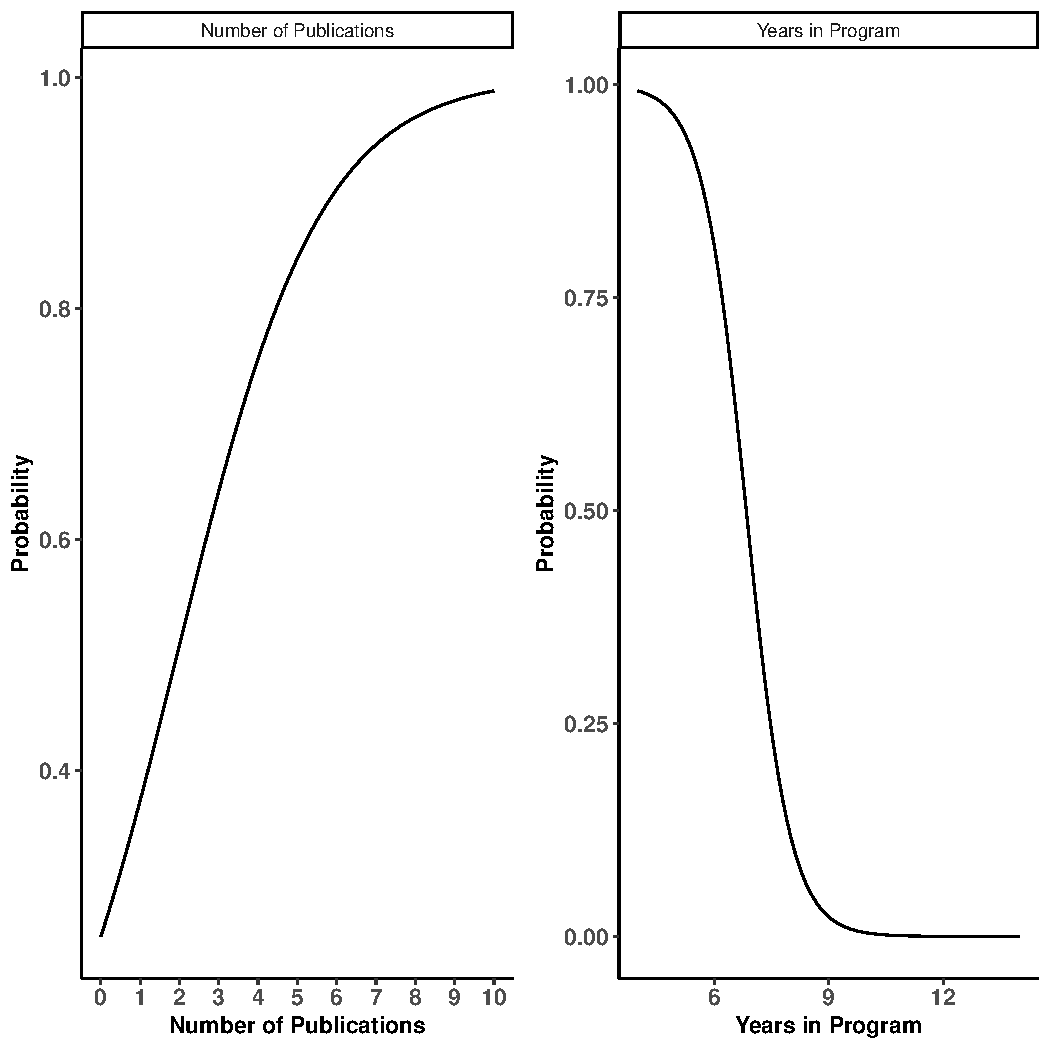
\includegraphics[width=\maxwidth]{figure/unnamed-chunk-4-1} 

\end{knitrout}

\section{Question 2}
Test a model that includes all two way interactions involving sex of applicant. For any significant interaction, construct a graph that shows the relationship between the relevant predictor and the probability of getting an interview, separately for men and women. Hold non graphed variables constant at their grand means and graph over the range of the target predictor.

\begin{knitrout}
\definecolor{shadecolor}{rgb}{0.969, 0.969, 0.969}\color{fgcolor}\begin{kframe}
\begin{alltt}
\hlstd{fit2}  \hlkwb{<-} \hlkwd{glm}\hlstd{(interview} \hlopt{~} \hlstd{sex} \hlopt{+} \hlstd{gre_c} \hlopt{+} \hlstd{pubs} \hlopt{+} \hlstd{years_c} \hlopt{+} \hlstd{sex}\hlopt{:}\hlstd{gre_c} \hlopt{+} \hlstd{sex}\hlopt{:}\hlstd{pubs} \hlopt{+} \hlstd{sex}\hlopt{:}\hlstd{years_c,}
             \hlkwc{data} \hlstd{= dat,} \hlkwc{family} \hlstd{=} \hlkwd{binomial}\hlstd{(}\hlstr{"logit"}\hlstd{))}
\hlkwd{cbind}\hlstd{(}\hlkwd{data.frame}\hlstd{(}\hlkwc{b} \hlstd{=} \hlkwd{coef}\hlstd{(fit2)),} \hlkwd{confint}\hlstd{(fit2))} \hlopt \hlkwd{data.frame}\hlstd{()} \hlopt
  \hlkwd{mutate}\hlstd{(}\hlkwc{term} \hlstd{=} \hlkwd{rownames}\hlstd{(.))} \hlopt
  \hlstd{tbl_df} \hlopt
  \hlkwd{select}\hlstd{(term,} \hlkwd{everything}\hlstd{())} \hlopt
  \hlkwd{setNames}\hlstd{(}\hlkwd{c}\hlstd{(}\hlstr{"term"}\hlstd{,} \hlstr{"b"}\hlstd{,} \hlstr{"lower"}\hlstd{,} \hlstr{"upper"}\hlstd{))} \hlopt
  \hlkwd{mutate}\hlstd{(}\hlkwc{sig} \hlstd{=} \hlkwd{ifelse}\hlstd{(}\hlkwd{sign}\hlstd{(lower)} \hlopt{==} \hlkwd{sign}\hlstd{(upper),} \hlstr{"sig"}\hlstd{,} \hlstr{"ns"}\hlstd{),}
         \hlkwc{CI} \hlstd{=} \hlkwd{sprintf}\hlstd{(}\hlstr{"[%.2f, %.2f]"}\hlstd{, lower, upper),} \hlkwc{b} \hlstd{=} \hlkwd{sprintf}\hlstd{(}\hlstr{"%.2f"}\hlstd{, b),}
         \hlkwc{term} \hlstd{=} \hlkwd{str_replace_all}\hlstd{(term,} \hlstr{"\textbackslash{}\textbackslash{}_"}\hlstd{,} \hlstr{"\textbackslash{}\textbackslash{}\textbackslash{}\textbackslash{}_"}\hlstd{))} \hlopt
  \hlkwd{mutate_at}\hlstd{(}\hlkwd{vars}\hlstd{(b, CI),} \hlkwd{funs}\hlstd{(}\hlkwd{ifelse}\hlstd{(sig} \hlopt{==} \hlstr{"sig"}\hlstd{,} \hlkwd{sprintf}\hlstd{(}\hlstr{"\textbackslash{}\textbackslash{}textbf\{%s\}"}\hlstd{, .), .)))} \hlopt
  \hlkwd{select}\hlstd{(term, b, CI)} \hlopt
  \hlkwd{kable}\hlstd{(.,} \hlstr{"latex"}\hlstd{,} \hlkwc{booktabs} \hlstd{= T,} \hlkwc{escape} \hlstd{= F)} \hlopt
  \hlkwd{kable_styling}\hlstd{(}\hlkwc{full_width} \hlstd{= F)}
\end{alltt}
\end{kframe}\begin{table}[H]
\centering
\begin{tabular}{lll}
\toprule
term & b & CI\\
\midrule
(Intercept) & -0.77 & [-1.80, 0.18]\\
sex & -0.93 & [-2.97, 0.84]\\
gre\_c & -0.00 & [-0.01, 0.00]\\
pubs & \textbf{0.49} & \textbf{[0.30, 0.72]}\\
years\_c & \textbf{-1.79} & \textbf{[-2.31, -1.38]}\\
\addlinespace
sex:gre\_c & -0.00 & [-0.01, 0.00]\\
sex:pubs & 0.19 & [-0.20, 0.64]\\
sex:years\_c & 0.06 & [-0.68, 0.77]\\
\bottomrule
\end{tabular}
\end{table}


\end{knitrout}

There were no significant 2 way interactions were significant

\section{Question 3}
Now add the ramining two way interactions. If any are significant, provide surface plots showing the relationship between the predictors (over their ranges) and the probability of getting an interview. Explain the nature of any significant interactions you graph.

\begin{knitrout}
\definecolor{shadecolor}{rgb}{0.969, 0.969, 0.969}\color{fgcolor}\begin{kframe}
\begin{alltt}
\hlkwd{cbind}\hlstd{(}\hlkwd{data.frame}\hlstd{(}\hlkwc{b} \hlstd{=} \hlkwd{coef}\hlstd{(fit3)),} \hlkwd{confint}\hlstd{(fit3))} \hlopt
  \hlkwd{data.frame}\hlstd{()} \hlopt
  \hlkwd{mutate}\hlstd{(}\hlkwc{term} \hlstd{=} \hlkwd{rownames}\hlstd{(.))} \hlopt
  \hlstd{tbl_df} \hlopt
  \hlkwd{select}\hlstd{(term,} \hlkwd{everything}\hlstd{())} \hlopt
  \hlkwd{setNames}\hlstd{(}\hlkwd{c}\hlstd{(}\hlstr{"term"}\hlstd{,} \hlstr{"b"}\hlstd{,} \hlstr{"lower"}\hlstd{,} \hlstr{"upper"}\hlstd{))} \hlopt
  \hlkwd{mutate}\hlstd{(}\hlkwc{sig} \hlstd{=} \hlkwd{ifelse}\hlstd{(}\hlkwd{sign}\hlstd{(lower)} \hlopt{==} \hlkwd{sign}\hlstd{(upper),} \hlstr{"sig"}\hlstd{,} \hlstr{"ns"}\hlstd{),}
         \hlkwc{CI} \hlstd{=} \hlkwd{sprintf}\hlstd{(}\hlstr{"[%.2f, %.2f]"}\hlstd{, lower, upper),} \hlkwc{b} \hlstd{=} \hlkwd{sprintf}\hlstd{(}\hlstr{"%.2f"}\hlstd{, b),}
         \hlkwc{term} \hlstd{=} \hlkwd{str_replace_all}\hlstd{(term,} \hlstr{"\textbackslash{}\textbackslash{}_"}\hlstd{,} \hlstr{"\textbackslash{}\textbackslash{}\textbackslash{}\textbackslash{}_"}\hlstd{))} \hlopt
  \hlkwd{mutate_at}\hlstd{(}\hlkwd{vars}\hlstd{(b, CI),} \hlkwd{funs}\hlstd{(}\hlkwd{ifelse}\hlstd{(sig} \hlopt{==} \hlstr{"sig"}\hlstd{,} \hlkwd{sprintf}\hlstd{(}\hlstr{"\textbackslash{}\textbackslash{}textbf\{%s\}"}\hlstd{, .), .)))} \hlopt
  \hlkwd{select}\hlstd{(term, b, CI)} \hlopt
  \hlkwd{kable}\hlstd{(.,} \hlstr{"latex"}\hlstd{,} \hlkwc{booktabs} \hlstd{= T,} \hlkwc{escape} \hlstd{= F)} \hlopt
  \hlkwd{kable_styling}\hlstd{(}\hlkwc{full_width} \hlstd{= F)}
\end{alltt}


{\ttfamily\noindent\bfseries\color{errorcolor}{\#\# Error in coef(fit3): object 'fit3' not found}}\begin{alltt}
\hlstd{fit3}  \hlkwb{<-} \hlkwd{glm}\hlstd{(interview} \hlopt{~} \hlstd{sex} \hlopt{+} \hlstd{gre_c} \hlopt{+} \hlstd{pubs} \hlopt{+} \hlstd{years_c} \hlopt{+} \hlstd{sex}\hlopt{:}\hlstd{gre_c} \hlopt{+} \hlstd{sex}\hlopt{:}\hlstd{pubs} \hlopt{+} \hlstd{sex}\hlopt{:}\hlstd{years_c} \hlopt{+}
               \hlstd{gre_c}\hlopt{:}\hlstd{pubs} \hlopt{+} \hlstd{gre_c}\hlopt{:}\hlstd{years_c} \hlopt{+} \hlstd{pubs}\hlopt{:}\hlstd{years_c,}
             \hlkwc{data} \hlstd{= dat,} \hlkwc{family} \hlstd{=} \hlkwd{binomial}\hlstd{(}\hlstr{"logit"}\hlstd{))}

\hlkwd{crossing}\hlstd{(}\hlkwc{sex} \hlstd{=} \hlkwd{mean}\hlstd{(dat}\hlopt{$}\hlstd{sex),}
         \hlkwc{gre_c} \hlstd{=} \hlkwd{mean}\hlstd{(dat}\hlopt{$}\hlstd{gre),}
         \hlkwc{pubs} \hlstd{=} \hlkwd{seq}\hlstd{(}\hlkwd{min}\hlstd{(dat}\hlopt{$}\hlstd{pubs),} \hlkwd{max}\hlstd{(dat}\hlopt{$}\hlstd{pubs),} \hlnum{.1}\hlstd{),}
         \hlkwc{years_c} \hlstd{=} \hlkwd{seq}\hlstd{(}\hlkwd{min}\hlstd{(dat}\hlopt{$}\hlstd{years_c),} \hlkwd{max}\hlstd{(dat}\hlopt{$}\hlstd{years_c),} \hlnum{.1}\hlstd{))} \hlopt
  \hlkwd{mutate}\hlstd{(}\hlkwc{pred} \hlstd{=} \hlkwd{predict}\hlstd{(fit3,} \hlkwc{newdata} \hlstd{= .),}
         \hlkwc{prob} \hlstd{=} \hlkwd{exp}\hlstd{(pred)}\hlopt{/}\hlstd{(}\hlnum{1} \hlopt{+} \hlkwd{exp}\hlstd{(pred)))} \hlopt
  \hlkwd{ggplot}\hlstd{(}\hlkwd{aes}\hlstd{(}\hlkwc{x} \hlstd{= years_c,} \hlkwc{y} \hlstd{= pubs,} \hlkwc{fill} \hlstd{= prob))} \hlopt{+}
    \hlcom{# scale_x_continuous(limits = c(0,10), breaks = seq(0,10,1)) +}
    \hlkwd{geom_raster}\hlstd{()} \hlopt{+}
    \hlkwd{labs}\hlstd{(}\hlkwc{x} \hlstd{=} \hlstr{"Years in Program"}\hlstd{,} \hlkwc{y} \hlstd{=} \hlstr{"Number of Publications"}\hlstd{)} \hlopt{+}
    \hlkwd{theme_classic}\hlstd{()} \hlopt{+}
    \hlkwd{theme}\hlstd{(}\hlkwc{axis.text} \hlstd{=} \hlkwd{element_text}\hlstd{(}\hlkwc{face} \hlstd{=} \hlstr{"bold"}\hlstd{,} \hlkwc{size} \hlstd{=} \hlkwd{rel}\hlstd{(}\hlnum{1}\hlstd{)),}
          \hlkwc{axis.title} \hlstd{=} \hlkwd{element_text}\hlstd{(}\hlkwc{face} \hlstd{=} \hlstr{"bold"}\hlstd{,} \hlkwc{size} \hlstd{=} \hlkwd{rel}\hlstd{(}\hlnum{1}\hlstd{)))}
\end{alltt}
\end{kframe}
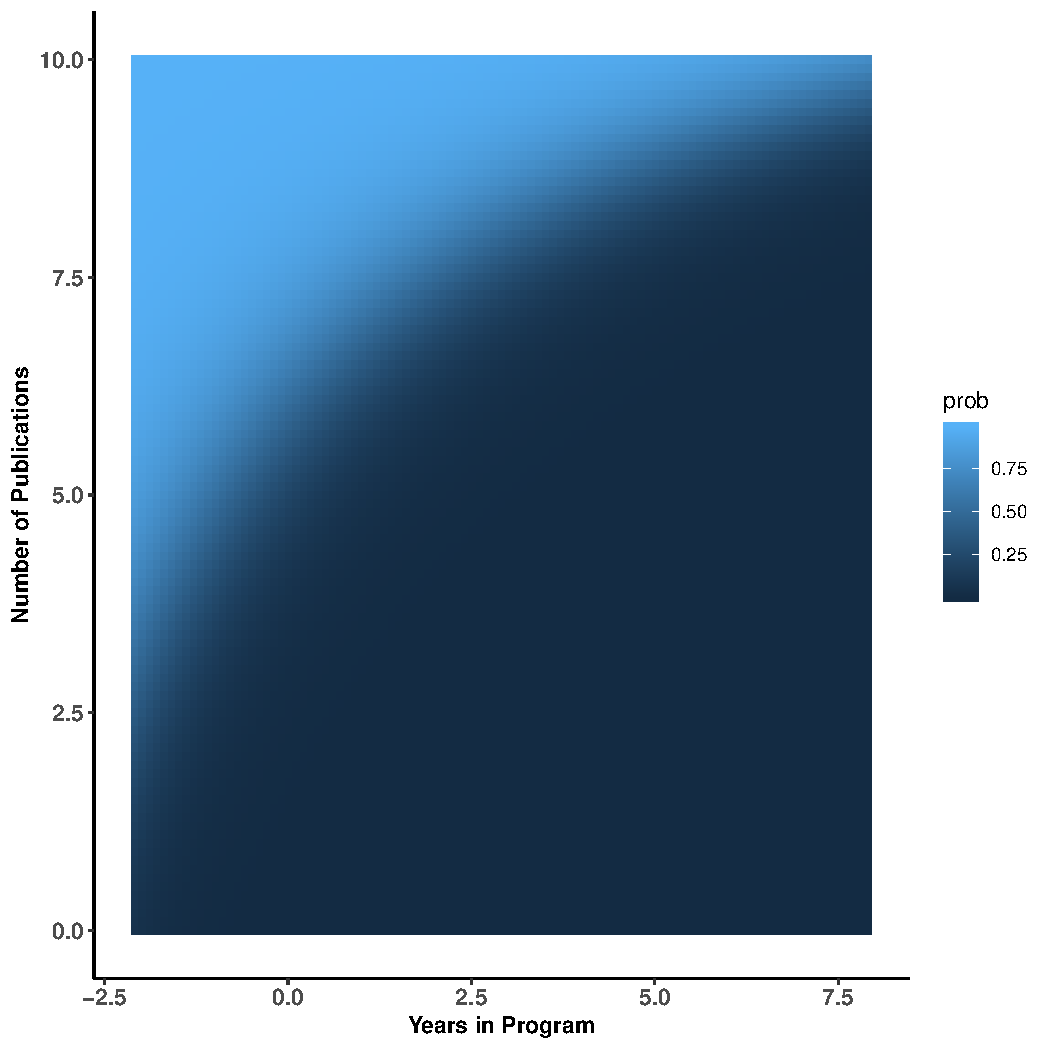
\includegraphics[width=\maxwidth]{figure/unnamed-chunk-6-1} 

\end{knitrout}

There was an interaction between the number of publications and the number of years in the program, such that as you spend more time in graduate school, you are going to need more publications to have an equal probability of getting an interview as someone who spent less time in graduate school.

\section{Question 4}
Finally, add to the basic model from Question 1, terms that test the quadratic effects of each continuous predictor. If any are significant, construct graphs showing the relationship between the predictor and the probability of getting an interview. Hold non- graphed variables constant at their grand means and graph over the range of the target predictor. Anything unusual about these graphs? Can you explain it?

\begin{knitrout}
\definecolor{shadecolor}{rgb}{0.969, 0.969, 0.969}\color{fgcolor}\begin{kframe}
\begin{alltt}
\hlstd{dat} \hlkwb{<-} \hlstd{dat} \hlopt
      \hlkwd{mutate_at}\hlstd{(}\hlkwd{vars}\hlstd{(gre_c, pubs, years_c),} \hlkwd{funs}\hlstd{(}\hlkwc{`2`} \hlstd{= .}\hlopt{^}\hlnum{2}\hlstd{))}
\hlstd{fit4}  \hlkwb{<-} \hlkwd{glm}\hlstd{(interview} \hlopt{~} \hlstd{sex} \hlopt{+} \hlstd{gre_c} \hlopt{+} \hlstd{pubs} \hlopt{+} \hlstd{years_c} \hlopt{+} \hlstd{gre_c_2} \hlopt{+} \hlstd{pubs_2} \hlopt{+} \hlstd{years_c_2,}
             \hlkwc{data} \hlstd{= dat,} \hlkwc{family} \hlstd{=} \hlkwd{binomial}\hlstd{(}\hlstr{"logit"}\hlstd{))}
\hlkwd{cbind}\hlstd{(}\hlkwd{data.frame}\hlstd{(}\hlkwc{b} \hlstd{=} \hlkwd{coef}\hlstd{(fit4)),} \hlkwd{confint}\hlstd{(fit4))} \hlopt \hlkwd{data.frame}\hlstd{()} \hlopt
  \hlkwd{mutate}\hlstd{(}\hlkwc{term} \hlstd{=} \hlkwd{rownames}\hlstd{(.))} \hlopt
  \hlstd{tbl_df} \hlopt
  \hlkwd{select}\hlstd{(term,} \hlkwd{everything}\hlstd{())} \hlopt
  \hlkwd{setNames}\hlstd{(}\hlkwd{c}\hlstd{(}\hlstr{"term"}\hlstd{,} \hlstr{"b"}\hlstd{,} \hlstr{"lower"}\hlstd{,} \hlstr{"upper"}\hlstd{))} \hlopt
  \hlkwd{mutate}\hlstd{(}\hlkwc{sig} \hlstd{=} \hlkwd{ifelse}\hlstd{(}\hlkwd{sign}\hlstd{(lower)} \hlopt{==} \hlkwd{sign}\hlstd{(upper),} \hlstr{"sig"}\hlstd{,} \hlstr{"ns"}\hlstd{),}
         \hlkwc{CI} \hlstd{=} \hlkwd{sprintf}\hlstd{(}\hlstr{"[%.2f, %.2f]"}\hlstd{, lower, upper),} \hlkwc{b} \hlstd{=} \hlkwd{sprintf}\hlstd{(}\hlstr{"%.2f"}\hlstd{, b),}
         \hlkwc{term} \hlstd{=} \hlkwd{str_replace_all}\hlstd{(term,} \hlstr{"\textbackslash{}\textbackslash{}_"}\hlstd{,} \hlstr{"\textbackslash{}\textbackslash{}\textbackslash{}\textbackslash{}_"}\hlstd{))} \hlopt
  \hlkwd{mutate_at}\hlstd{(}\hlkwd{vars}\hlstd{(b, CI),} \hlkwd{funs}\hlstd{(}\hlkwd{ifelse}\hlstd{(sig} \hlopt{==} \hlstr{"sig"}\hlstd{,} \hlkwd{sprintf}\hlstd{(}\hlstr{"\textbackslash{}\textbackslash{}textbf\{%s\}"}\hlstd{, .), .)))} \hlopt
  \hlkwd{select}\hlstd{(term, b, CI)} \hlopt
  \hlkwd{kable}\hlstd{(.,} \hlstr{"latex"}\hlstd{,} \hlkwc{booktabs} \hlstd{= T,} \hlkwc{escape} \hlstd{= F)} \hlopt
  \hlkwd{kable_styling}\hlstd{(}\hlkwc{full_width} \hlstd{= F)}
\end{alltt}
\end{kframe}\begin{table}[H]
\centering
\begin{tabular}{lll}
\toprule
term & b & CI\\
\midrule
(Intercept) & \textbf{-2.96} & \textbf{[-4.79, -1.42]}\\
sex & -0.12 & [-0.92, 0.67]\\
gre\_c & -0.00 & [-0.01, 0.00]\\
pubs & \textbf{1.64} & \textbf{[0.99, 2.39]}\\
years\_c & \textbf{-2.09} & \textbf{[-2.60, -1.66]}\\
\addlinespace
gre\_c\_2 & -0.00 & [-0.00, 0.00]\\
pubs\_2 & \textbf{-0.12} & \textbf{[-0.19, -0.05]}\\
years\_c\_2 & \textbf{0.21} & \textbf{[0.09, 0.30]}\\
\bottomrule
\end{tabular}
\end{table}

\begin{kframe}\begin{alltt}
\hlcom{# pubs}
\hlstd{p1} \hlkwb{<-} \hlkwd{crossing}\hlstd{(}\hlkwc{sex} \hlstd{=} \hlkwd{mean}\hlstd{(dat}\hlopt{$}\hlstd{sex),}
         \hlkwc{gre_c} \hlstd{=} \hlnum{0}\hlstd{,}
         \hlkwc{pubs} \hlstd{=} \hlkwd{seq}\hlstd{(}\hlkwd{min}\hlstd{(dat}\hlopt{$}\hlstd{pubs),} \hlkwd{max}\hlstd{(dat}\hlopt{$}\hlstd{pubs),} \hlnum{.1}\hlstd{),}
         \hlkwc{years_c} \hlstd{=} \hlnum{0}\hlstd{)} \hlopt
  \hlkwd{mutate_at}\hlstd{(}\hlkwd{vars}\hlstd{(gre_c, pubs, years_c),} \hlkwd{funs}\hlstd{(}\hlkwc{`2`} \hlstd{= .}\hlopt{^}\hlnum{2}\hlstd{))} \hlopt
  \hlkwd{mutate}\hlstd{(}\hlkwc{pred} \hlstd{=} \hlkwd{predict}\hlstd{(fit4,} \hlkwc{newdata} \hlstd{= .),}
         \hlkwc{prob} \hlstd{=} \hlkwd{exp}\hlstd{(pred)}\hlopt{/}\hlstd{(}\hlnum{1} \hlopt{+} \hlkwd{exp}\hlstd{(pred)),}
         \hlkwc{p} \hlstd{=} \hlstr{"Number of Publications"}\hlstd{)} \hlopt
  \hlkwd{ggplot}\hlstd{(}\hlkwd{aes}\hlstd{(}\hlkwc{x} \hlstd{= pubs,} \hlkwc{y} \hlstd{= prob))} \hlopt{+}
    \hlkwd{scale_x_continuous}\hlstd{(}\hlkwc{limits} \hlstd{=} \hlkwd{c}\hlstd{(}\hlnum{0}\hlstd{,}\hlnum{10}\hlstd{),} \hlkwc{breaks} \hlstd{=} \hlkwd{seq}\hlstd{(}\hlnum{0}\hlstd{,}\hlnum{10}\hlstd{,}\hlnum{1}\hlstd{))} \hlopt{+}
    \hlkwd{geom_line}\hlstd{()} \hlopt{+}
    \hlkwd{labs}\hlstd{(}\hlkwc{x} \hlstd{=} \hlstr{"Number of Publications"}\hlstd{,} \hlkwc{y} \hlstd{=} \hlstr{"Probability"}\hlstd{)} \hlopt{+}
    \hlkwd{theme_classic}\hlstd{()} \hlopt{+}
    \hlkwd{facet_wrap}\hlstd{(}\hlopt{~}\hlstd{p)} \hlopt{+}
    \hlkwd{theme}\hlstd{(}\hlkwc{axis.text} \hlstd{=} \hlkwd{element_text}\hlstd{(}\hlkwc{face} \hlstd{=} \hlstr{"bold"}\hlstd{,} \hlkwc{size} \hlstd{=} \hlkwd{rel}\hlstd{(}\hlnum{1}\hlstd{)),}
          \hlkwc{axis.title} \hlstd{=} \hlkwd{element_text}\hlstd{(}\hlkwc{face} \hlstd{=} \hlstr{"bold"}\hlstd{,} \hlkwc{size} \hlstd{=} \hlkwd{rel}\hlstd{(}\hlnum{1}\hlstd{)))}


\hlcom{# years}
\hlstd{p2} \hlkwb{<-} \hlkwd{crossing}\hlstd{(}\hlkwc{sex} \hlstd{=} \hlkwd{mean}\hlstd{(dat}\hlopt{$}\hlstd{sex),}
         \hlkwc{gre_c} \hlstd{=} \hlnum{0}\hlstd{,}
         \hlkwc{pubs} \hlstd{=} \hlkwd{mean}\hlstd{(dat}\hlopt{$}\hlstd{pubs),}
         \hlkwc{years_c} \hlstd{=} \hlkwd{seq}\hlstd{(}\hlkwd{min}\hlstd{(dat}\hlopt{$}\hlstd{years_c),} \hlkwd{max}\hlstd{(dat}\hlopt{$}\hlstd{years_c),} \hlnum{.1}\hlstd{))} \hlopt
  \hlkwd{mutate_at}\hlstd{(}\hlkwd{vars}\hlstd{(gre_c, pubs, years_c),} \hlkwd{funs}\hlstd{(}\hlkwc{`2`} \hlstd{= .}\hlopt{^}\hlnum{2}\hlstd{))} \hlopt
  \hlkwd{mutate}\hlstd{(}\hlkwc{pred} \hlstd{=} \hlkwd{predict}\hlstd{(fit4,} \hlkwc{newdata} \hlstd{= .),}
         \hlkwc{prob} \hlstd{=} \hlkwd{exp}\hlstd{(pred)}\hlopt{/}\hlstd{(}\hlnum{1} \hlopt{+} \hlkwd{exp}\hlstd{(pred)),}
         \hlkwc{p} \hlstd{=} \hlstr{"Years in Program"}\hlstd{)} \hlopt
  \hlkwd{ggplot}\hlstd{(}\hlkwd{aes}\hlstd{(}\hlkwc{x} \hlstd{= years_c,} \hlkwc{y} \hlstd{= prob))} \hlopt{+}
    \hlcom{# scale_x_continuous(limits = c(0,10), breaks = seq(0,10,1)) +}
    \hlkwd{geom_line}\hlstd{()} \hlopt{+}
    \hlkwd{labs}\hlstd{(}\hlkwc{x} \hlstd{=} \hlstr{"Years in Program"}\hlstd{,} \hlkwc{y} \hlstd{=} \hlstr{"Probability"}\hlstd{)} \hlopt{+}
    \hlkwd{theme_classic}\hlstd{()} \hlopt{+}
    \hlkwd{facet_wrap}\hlstd{(}\hlopt{~}\hlstd{p)} \hlopt{+}
    \hlkwd{theme}\hlstd{(}\hlkwc{axis.text} \hlstd{=} \hlkwd{element_text}\hlstd{(}\hlkwc{face} \hlstd{=} \hlstr{"bold"}\hlstd{,} \hlkwc{size} \hlstd{=} \hlkwd{rel}\hlstd{(}\hlnum{1}\hlstd{)),}
          \hlkwc{axis.title} \hlstd{=} \hlkwd{element_text}\hlstd{(}\hlkwc{face} \hlstd{=} \hlstr{"bold"}\hlstd{,} \hlkwc{size} \hlstd{=} \hlkwd{rel}\hlstd{(}\hlnum{1}\hlstd{)))}

\hlstd{gridExtra}\hlopt{::}\hlkwd{grid.arrange}\hlstd{(p1, p2,} \hlkwc{nrow} \hlstd{=} \hlnum{1}\hlstd{)}
\end{alltt}
\end{kframe}
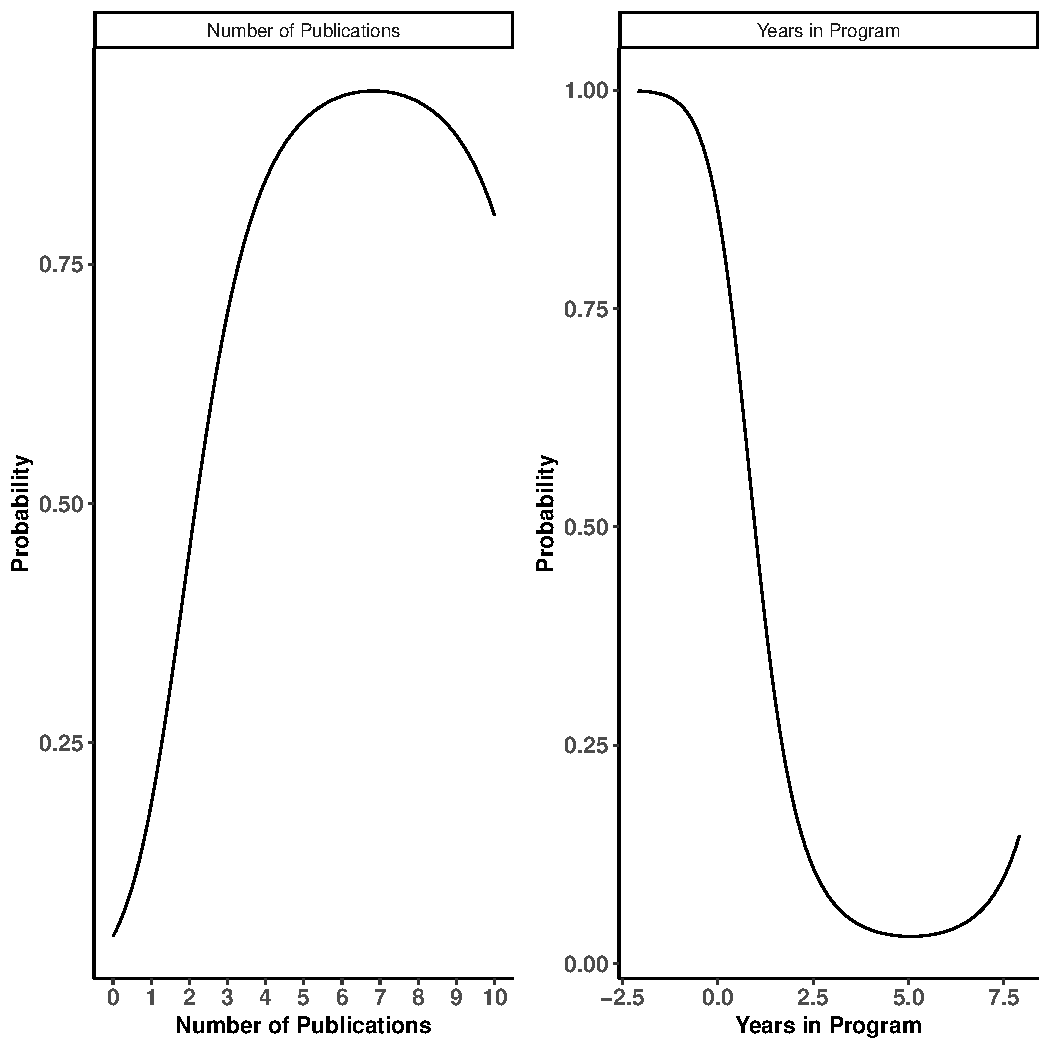
\includegraphics[width=\maxwidth]{figure/unnamed-chunk-7-1} 

\end{knitrout}

In both graphs, the high end of publications and years in program see a reversal in the probability of an interview. For number of publications, you actually see a decreased when publications raise above 7 and for years in program, you see the probability go slightly up when you spend 5 years longer in graduate school than the average student. 

For number of publications, this may be because the number reflects lots of second author publications and fewer first author publications or the publications may have been in lower tier journals. For years in the program, it may be that the people who took much longer (> 5+ additional years) than others took time off to start a family, work in industry, etc., while those taking an additional 1 to 5 years may have been less productive while actually in school. 

However, both of these could be measurement error because there are fewer observations at the tails of both distributions of the predictors.
\end{document}
